\begin{figure}[htbp]
\centering
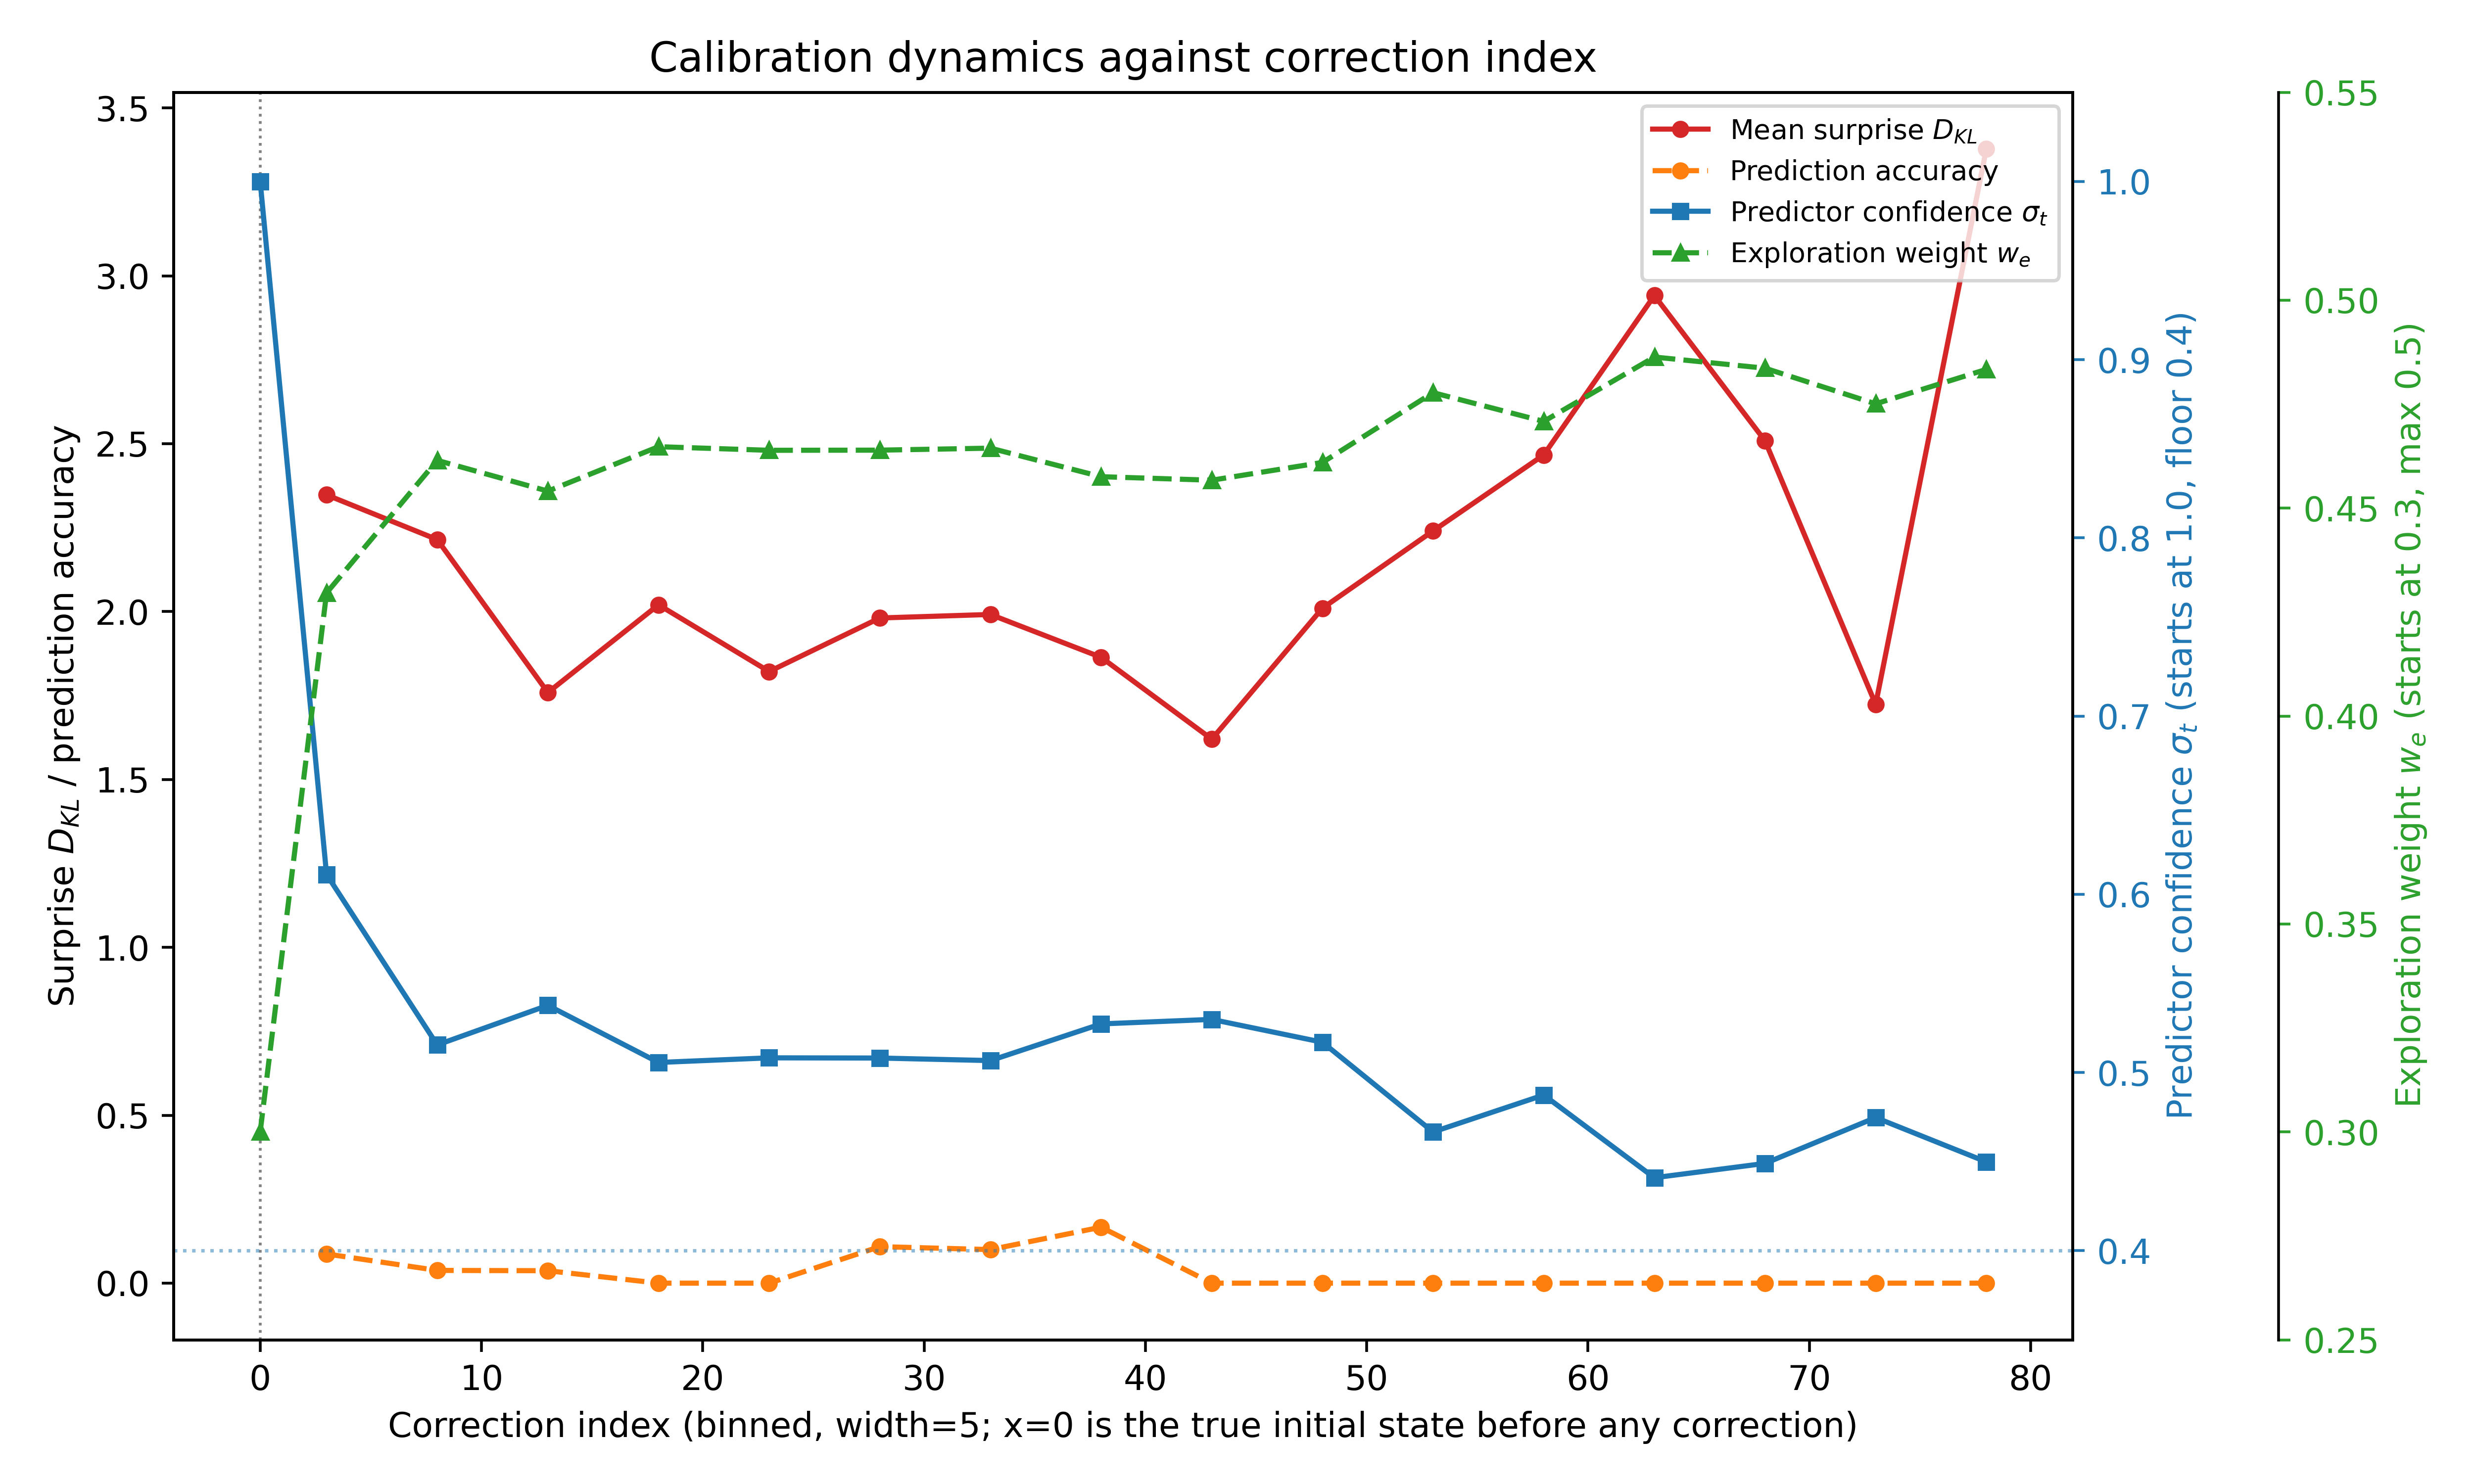
\includegraphics[width=0.88\linewidth]{figures/figure3.png}
\caption{Calibration dynamics: surprise, accuracy, uncertainty vs. correction index}
\label{fig:calibration}
\end{figure}
\section{Conclusion}

We introduced PEC-Nav, a self-calibrating frontier search for embodied question answering. The insight is that prediction errors are more useful than predictions, since measuring surprise between anticipated and observed layouts lets the agent adapt its confidence and exploration balance within an episode, untrained. On LMEE-Bench's 58-task subset it reaches 24.45\% SR, 16.86 SPL, 57.93 MLLM-Score and 66.21\% QA accuracy, and across three ablations the loop improves success and path efficiency while the predictor alone does not. The evidence is directional rather than resolved. Next steps include a learned detector in place of the semantic sensor, a fixed-scalar control separating calibration from shrinkage, and a static baseline at full scale.
